\documentclass[12pt,a4paper]{article}

\usepackage[utf8]{inputenc}
\usepackage[spanish]{babel}
\usepackage{graphicx}
\usepackage{geometry}
\geometry{a4paper, margin=2.5cm}
\usepackage{xcolor}
\usepackage{listings}
\usepackage{booktabs}
\usepackage{amsmath}
\usepackage{subcaption}
\usepackage{float}
\usepackage[colorlinks=true, linkcolor=blue, urlcolor=blue]{hyperref}

\definecolor{codegreen}{rgb}{0,0.6,0}
\definecolor{codegray}{rgb}{0.5,0.5,0.5}
\definecolor{codepurple}{rgb}{0.58,0,0.82}
\definecolor{backcolour}{rgb}{0.95,0.95,0.92}

\lstdefinestyle{mystyle}{
    backgroundcolor=\color{backcolour},   
    commentstyle=\color{codegreen},
    keywordstyle=\color{magenta},
    numberstyle=\tiny\color{codegray},
    stringstyle=\color{codepurple},
    basicstyle=\ttfamily\footnotesize,
    breakatwhitespace=false,         
    breaklines=true,                 
    captionpos=b,                    
    keepspaces=true,                 
    numbers=left,                    
    numbersep=5pt,                  
    showspaces=false,                
    showstringspaces=false,
    showtabs=false,                  
    tabsize=2,
    literate={á}{{\'a}}1 {é}{{\'e}}1 {í}{{\'i}}1 {ó}{{\'o}}1 {ú}{{\'u}}1
             {Á}{{\'A}}1 {É}{{\'E}}1 {Í}{{\'I}}1 {Ó}{{\'O}}1 {Ú}{{\'U}}1
             {ñ}{{\~n}}1 {Ñ}{{\~N}}1
}
\lstset{style=mystyle}

\title{\Huge\textbf{PROYECTO ESP32} \\ \Large Control de LED y Monitoreo de Potenciómetro vía WiFi \\ \vspace{0.5cm} \normalsize \textit{Servidor web embebido con interfaz gráfica, control On/Off y gauge de voltaje en tiempo real}}
\author{Msc. Néstor Fabio Montoya Palacios}
\date{2026 \\ \vspace{0.2cm} \small Plataforma: ESP32 Dev Module}

\begin{document}

\maketitle
\tableofcontents
\newpage

% ══════════════════════════════════════════════════════════════
\section{Introducción}
% ══════════════════════════════════════════════════════════════

Este documento describe el proyecto ``Control de LED y Monitoreo de Potenciómetro vía WiFi'', que convierte el ESP32 en un \textbf{servidor web local} capaz de servir una página HTML completa con interfaz gráfica interactiva. El sistema permite \textbf{encender y apagar un LED} desde el navegador mediante un interruptor estilo industrial, y simultáneamente \textbf{monitorear en tiempo real el voltaje} de un potenciómetro a través de un gauge (medidor tipo reloj) generado con Google Charts.

A diferencia de los proyectos anteriores que utilizaban comunicación serial o Bluetooth, este proyecto introduce el paradigma de \textbf{Internet de las Cosas (IoT)}: el ESP32 se conecta a una red WiFi existente, obtiene una dirección IP y sirve una aplicación web completa accesible desde cualquier dispositivo conectado a la misma red. La página web se almacena en la memoria Flash del ESP32 mediante la directiva \texttt{PROGMEM} y utiliza tecnologías web modernas como CSS3, JavaScript asíncrono y la API Fetch para comunicarse con el microcontrolador.

% ══════════════════════════════════════════════════════════════
\section{Objetivo del Proyecto}
% ══════════════════════════════════════════════════════════════

Implementar un sistema IoT con servidor web embebido en el ESP32 que:
\begin{itemize}
    \item Conecte el ESP32 a una red WiFi doméstica como cliente (modo estación).
    \item Sirva una página web completa con HTML, CSS y JavaScript desde la memoria Flash.
    \item Permita \textbf{encender y apagar un LED} mediante un interruptor visual en el navegador.
    \item Lea continuamente el potenciómetro (GPIO34) y exponga los datos como API REST en formato JSON.
    \item Muestre un \textbf{gauge de voltaje} en tiempo real usando Google Charts.
    \item Presente los valores numéricos de ADC, voltaje y porcentaje actualizados cada 500\,ms.
    \item Sea accesible desde cualquier dispositivo (computador, celular, tablet) en la misma red.
\end{itemize}

% ══════════════════════════════════════════════════════════════
\section{Materiales Necesarios}
% ══════════════════════════════════════════════════════════════

\begin{table}[h!]
\centering
\begin{tabular}{cll}
\toprule
\textbf{Cant.} & \textbf{Componente} & \textbf{Especificación} \\
\midrule
1 & ESP32 Dev Module & Microcontrolador dual-core con Wi-Fi/Bluetooth \\
1 & Potenciómetro & 10\,k$\Omega$ lineal, 3 terminales \\
1 & LED & Diodo emisor de luz, 5\,mm \\
1 & Resistencia & 220\,$\Omega$ (limitadora de corriente) \\
1 & Protoboard & Placa de pruebas de 830 puntos \\
  & Cables jumper & Macho-macho para conexiones \\
1 & Cable USB & Para programación y alimentación \\
1 & Red WiFi & Router con acceso a la red local \\
1 & Navegador web & Chrome, Firefox o cualquier navegador moderno \\
\bottomrule
\end{tabular}
\caption{Lista de materiales del proyecto Potenciómetro WiFi}
\end{table}

% ══════════════════════════════════════════════════════════════
\section{Esquema de Conexión}
% ══════════════════════════════════════════════════════════════

El circuito es idéntico al de los proyectos anteriores de potenciómetro. El potenciómetro se conecta como divisor de voltaje entre 3,3\,V y GND, con su cursor en GPIO34 (entrada analógica). El LED se conecta a GPIO4 a través de una resistencia de 220\,$\Omega$. La comunicación WiFi no requiere hardware adicional ya que el ESP32 integra el módulo de radio en el propio chip.

\begin{figure}[H]
\centering
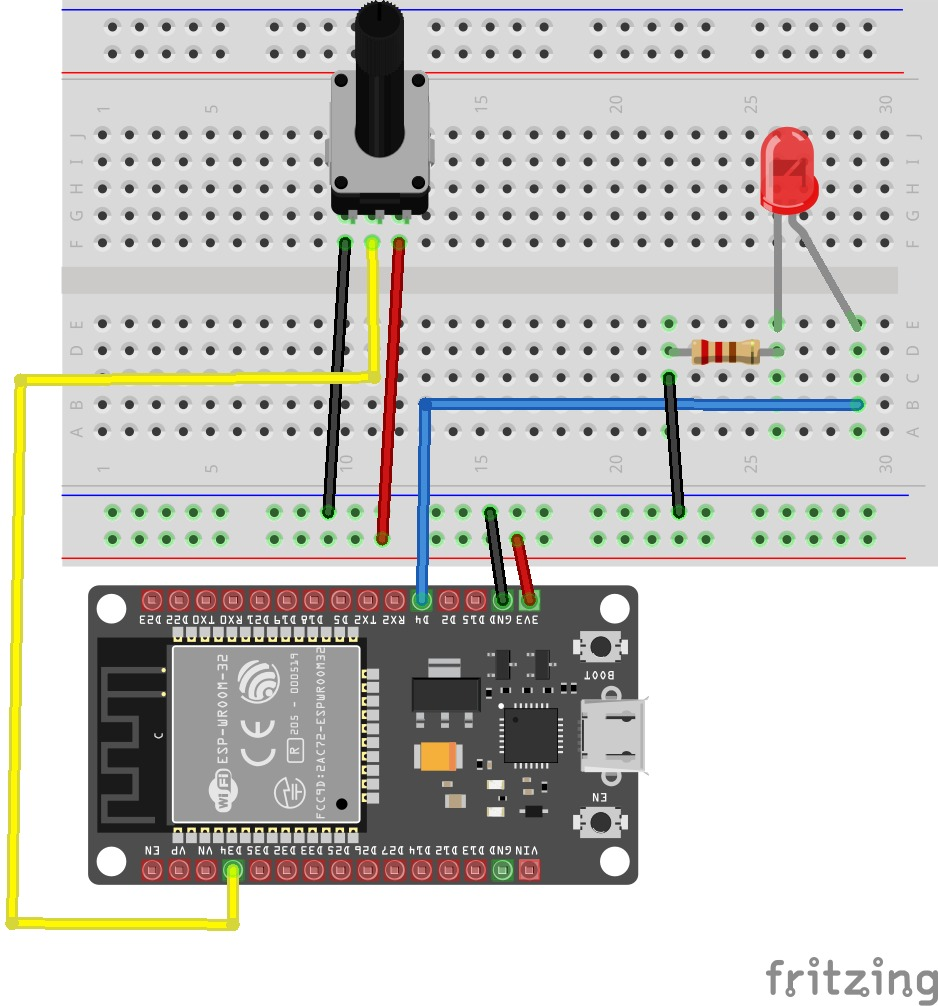
\includegraphics[width=0.85\textwidth]{../Esquemas/Potenciometro_esq.jpeg}
\caption{Esquema de conexión del circuito en Fritzing -- el WiFi es interno al ESP32}
\label{fig:esquema}
\end{figure}

\subsection{Diagrama de Conexiones}

\begin{center}
\begin{tabular}{lll}
\toprule
\textbf{Componente} & \textbf{Pin} & \textbf{ESP32 GPIO} \\
\midrule
Potenciómetro & Terminal 1 & 3.3V \\
Potenciómetro & Terminal 2 (cursor) & GPIO34 (ADC1\_CH6) \\
Potenciómetro & Terminal 3 & GND \\
Resistencia 220\,$\Omega$ & Terminal 1 & GPIO4 \\
LED & Ánodo (+) & Resistencia 220\,$\Omega$ (Terminal 2) \\
LED & Cátodo (--) & GND \\
\bottomrule
\end{tabular}
\end{center}

\textbf{Nota:} A diferencia de los proyectos con Bluetooth, en este caso el ESP32 utiliza su módulo WiFi integrado para crear un servidor web accesible desde la red local. No se requiere ningún componente adicional para la conectividad inalámbrica.

% ══════════════════════════════════════════════════════════════
\section{Código Fuente}
% ══════════════════════════════════════════════════════════════

A continuación se presenta el código completo del proyecto. Este programa combina funcionalidades de firmware embebido con desarrollo web frontend, ya que incluye HTML, CSS y JavaScript almacenados en la memoria Flash del ESP32.

\subsection{Código Completo}
\lstinputlisting[language=C++, title=Potenciometro\_y\_On\_Off\_Wifi.ino]{../Arduino/Potenciometro_y_On_Off_Wifi/Potenciometro_y_On_Off_Wifi.ino}

% ══════════════════════════════════════════════════════════════
\subsection{Análisis del Código}
% ══════════════════════════════════════════════════════════════

El código se divide en cuatro grandes bloques: configuración WiFi, página web embebida, funciones de manejo de peticiones y el ciclo principal.

\subsubsection*{Librerías y Configuración WiFi}

El programa incluye dos librerías fundamentales:
\begin{itemize}
    \item \textbf{\texttt{WiFi.h}:} Proporciona las funciones para conectar el ESP32 a una red WiFi como cliente (modo estación). Permite obtener la dirección IP asignada por el router.
    \item \textbf{\texttt{WebServer.h}:} Implementa un servidor HTTP ligero que puede responder a peticiones GET y POST. Se instancia en el puerto 80 (puerto HTTP estándar).
\end{itemize}

Se definen las credenciales de la red WiFi (\texttt{miSSID} y \texttt{miPASSWORD}), los pines del potenciómetro (GPIO34) y del LED (GPIO4), y una variable booleana \texttt{ledEncendido} para rastrear el estado del LED.

\subsubsection*{Página Web Embebida (PROGMEM)}

La constante \texttt{paginaWeb[]} almacena toda la interfaz web en la memoria Flash usando \texttt{PROGMEM} y la sintaxis de raw string literal \texttt{R"=====( ... )====="}. Esta página incluye:

\begin{itemize}
    \item \textbf{HTML:} Estructura con dos paneles (control del LED y gauge del potenciómetro) y un panel inferior con datos numéricos (valor ADC, voltaje y porcentaje).
    \item \textbf{CSS con glassmorphism:} Diseño moderno con gradientes, \texttt{backdrop-filter: blur()}, bordes semitransparentes y sombras multicapa. El interruptor del LED simula un switch industrial 3D con animaciones CSS puras.
    \item \textbf{JavaScript:} Utiliza Google Charts para renderizar un gauge de 0 a 3,3\,V con zonas de color (verde, amarillo, rojo). La función \texttt{actualizarDatos()} usa \texttt{fetch('/datos')} cada 500\,ms para obtener datos JSON del ESP32.
\end{itemize}

\subsubsection*{API REST del ESP32}

El servidor expone tres rutas (endpoints):

\begin{center}
\begin{tabular}{llp{7cm}}
\toprule
\textbf{Ruta} & \textbf{Método} & \textbf{Función} \\
\midrule
\texttt{/} & GET & Sirve la página HTML completa \\
\texttt{/datos} & GET & Retorna JSON con \texttt{adc}, \texttt{voltaje} y \texttt{porcentaje} \\
\texttt{/led?estado=on|off} & GET & Enciende o apaga el LED y confirma el estado \\
\bottomrule
\end{tabular}
\end{center}

\subsubsection*{Función \texttt{manejarDatos()}}

Esta función lee el ADC, calcula el voltaje y el porcentaje, y construye una respuesta JSON:
\begin{equation}
V = \frac{\text{valorADC} \times 3{,}3}{4095} \qquad \text{Porcentaje} = \texttt{map}(\text{valorADC}, 0, 4095, 0, 100)
\label{eq:voltaje}
\end{equation}

\subsubsection*{Función \texttt{setup()}}

\begin{enumerate}
    \item Inicia la comunicación serial a 115200 baudios.
    \item Configura GPIO34 como entrada y GPIO4 como salida (LED apagado al inicio).
    \item Conecta a la red WiFi usando \texttt{WiFi.begin()} y espera la conexión.
    \item Imprime la dirección IP asignada por el router.
    \item Registra las tres rutas del servidor con \texttt{servidor.on()}.
    \item Inicia el servidor HTTP con \texttt{servidor.begin()}.
\end{enumerate}

\subsubsection*{Función \texttt{loop()}}

El bucle principal es extremadamente simple: solo llama a \texttt{servidor.handleClient()} para atender las peticiones HTTP entrantes. Toda la lógica de lectura del potenciómetro se ejecuta bajo demanda cuando el navegador solicita datos.

% ══════════════════════════════════════════════════════════════
\section{Principio de Funcionamiento}
% ══════════════════════════════════════════════════════════════

\subsection{Arquitectura Cliente-Servidor}

Este proyecto implementa una arquitectura \textbf{cliente-servidor HTTP} donde el ESP32 actúa como servidor y el navegador web como cliente. El flujo de comunicación es:

\begin{enumerate}
    \item El ESP32 se conecta a la red WiFi y obtiene una IP (ej. \texttt{192.168.1.x}).
    \item El usuario abre esa IP en su navegador, generando una petición \texttt{GET /}.
    \item El ESP32 responde con la página HTML completa (almacenada en \texttt{PROGMEM}).
    \item El JavaScript de la página realiza peticiones \texttt{fetch('/datos')} cada 500\,ms.
    \item El ESP32 responde con un JSON: \texttt{\{"adc":1123, "voltaje":0.90, "porcentaje":27\}}.
    \item Cuando el usuario toca el interruptor, se envía \texttt{fetch('/led?estado=on')}.
    \item El ESP32 ejecuta \texttt{digitalWrite(pinLED, HIGH)} y confirma.
\end{enumerate}

\subsection{WiFi en el ESP32 (Modo Estación)}

El ESP32 integra un controlador WiFi 802.11 b/g/n que puede operar en tres modos:

\begin{center}
\begin{tabular}{lp{9cm}}
\toprule
\textbf{Modo} & \textbf{Descripción} \\
\midrule
Estación (STA) & Se conecta a un router existente como cliente (usado en este proyecto) \\
Punto de Acceso (AP) & Crea su propia red WiFi \\
Dual (STA+AP) & Ambos simultáneamente \\
\bottomrule
\end{tabular}
\end{center}

En modo estación, la librería \texttt{WiFi.h} proporciona:
\begin{itemize}
    \item \texttt{WiFi.begin(ssid, password)}: Inicia la conexión a la red.
    \item \texttt{WiFi.status()}: Devuelve el estado de la conexión (\texttt{WL\_CONNECTED}).
    \item \texttt{WiFi.localIP()}: Devuelve la dirección IP asignada por DHCP.
\end{itemize}

\subsection{Servidor Web con WebServer.h}

La librería \texttt{WebServer.h} implementa un servidor HTTP minimalista que permite:
\begin{itemize}
    \item \texttt{servidor.on("/ruta", funcion)}: Asocia una URL a una función callback.
    \item \texttt{servidor.send(codigo, tipo, contenido)}: Envía una respuesta HTTP.
    \item \texttt{servidor.arg("param")}: Obtiene parámetros de la URL (query string).
    \item \texttt{servidor.handleClient()}: Procesa la siguiente petición pendiente.
\end{itemize}

\subsection{Interfaz Web: Google Charts Gauge}

La página web utiliza la librería \textbf{Google Charts} (cargada vía CDN) para renderizar un gauge analógico que muestra el voltaje del potenciómetro en tiempo real. El gauge está configurado con tres zonas de color:

\begin{center}
\begin{tabular}{lcl}
\toprule
\textbf{Zona} & \textbf{Rango} & \textbf{Significado} \\
\midrule
Verde & 0 -- 1,8\,V & Voltaje bajo \\
Amarillo & 1,8 -- 2,7\,V & Voltaje medio \\
Rojo & 2,7 -- 3,3\,V & Voltaje alto \\
\bottomrule
\end{tabular}
\end{center}

\subsection{Cadena de Procesamiento}

\begin{verbatim}
    Potenciómetro        ADC 12-bit       JSON API        Navegador
    (ángulo)    ────>   (0 - 4095)  ────> /datos  ────>  fetch() JS
    0° - 270°            voltaje          HTTP GET        Google Charts
                        0 - 3.3 V                        Gauge + datos
                                                            │
                              ┌─────────────────────────────┤
                              v                             v
                        Interruptor web              Gauge de voltaje
                      (fetch /led?estado=)           + valores numéricos
                              │
                              v
                        digitalWrite()
                     (GPIO4: LED on/off)
\end{verbatim}

\subsection{El Potenciómetro como Divisor de Voltaje}

El potenciómetro actúa como divisor de voltaje ajustable. Con sus terminales extremos entre 3,3\,V y GND:

\begin{equation}
V_{\text{cursor}} = V_{CC} \times \frac{\theta}{\theta_{\max}} = 3{,}3 \times \frac{\theta}{270°}
\label{eq:divisor}
\end{equation}

% ══════════════════════════════════════════════════════════════
\section{Fotografías del Montaje}
% ══════════════════════════════════════════════════════════════

Las siguientes imágenes documentan el proyecto en funcionamiento, mostrando tanto la interfaz web como el montaje físico del circuito.

\begin{figure}[H]
\centering
\begin{subfigure}[b]{0.48\textwidth}
    \centering
    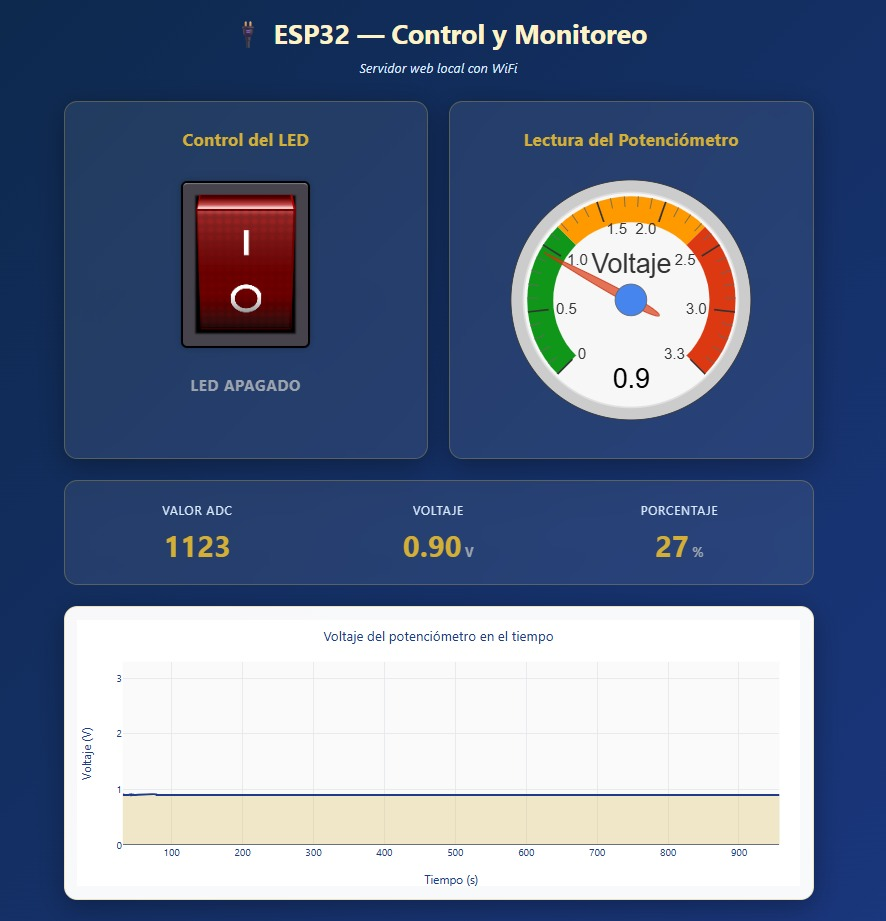
\includegraphics[width=\textwidth]{../Imagenes/Potenciometro_y_On_Off_Wifi_imgs/Potenciometro_y_On_Off_Wifi_img1.jpeg}
    \caption{Captura de la interfaz web mostrando el interruptor del LED apagado, gauge marcando 0,9\,V, y valores numéricos: ADC 1123, Voltaje 0,90\,V, Porcentaje 27\%. Se observa también la gráfica de voltaje en el tiempo.}
    \label{fig:wifi1}
\end{subfigure}
\hfill
\begin{subfigure}[b]{0.48\textwidth}
    \centering
    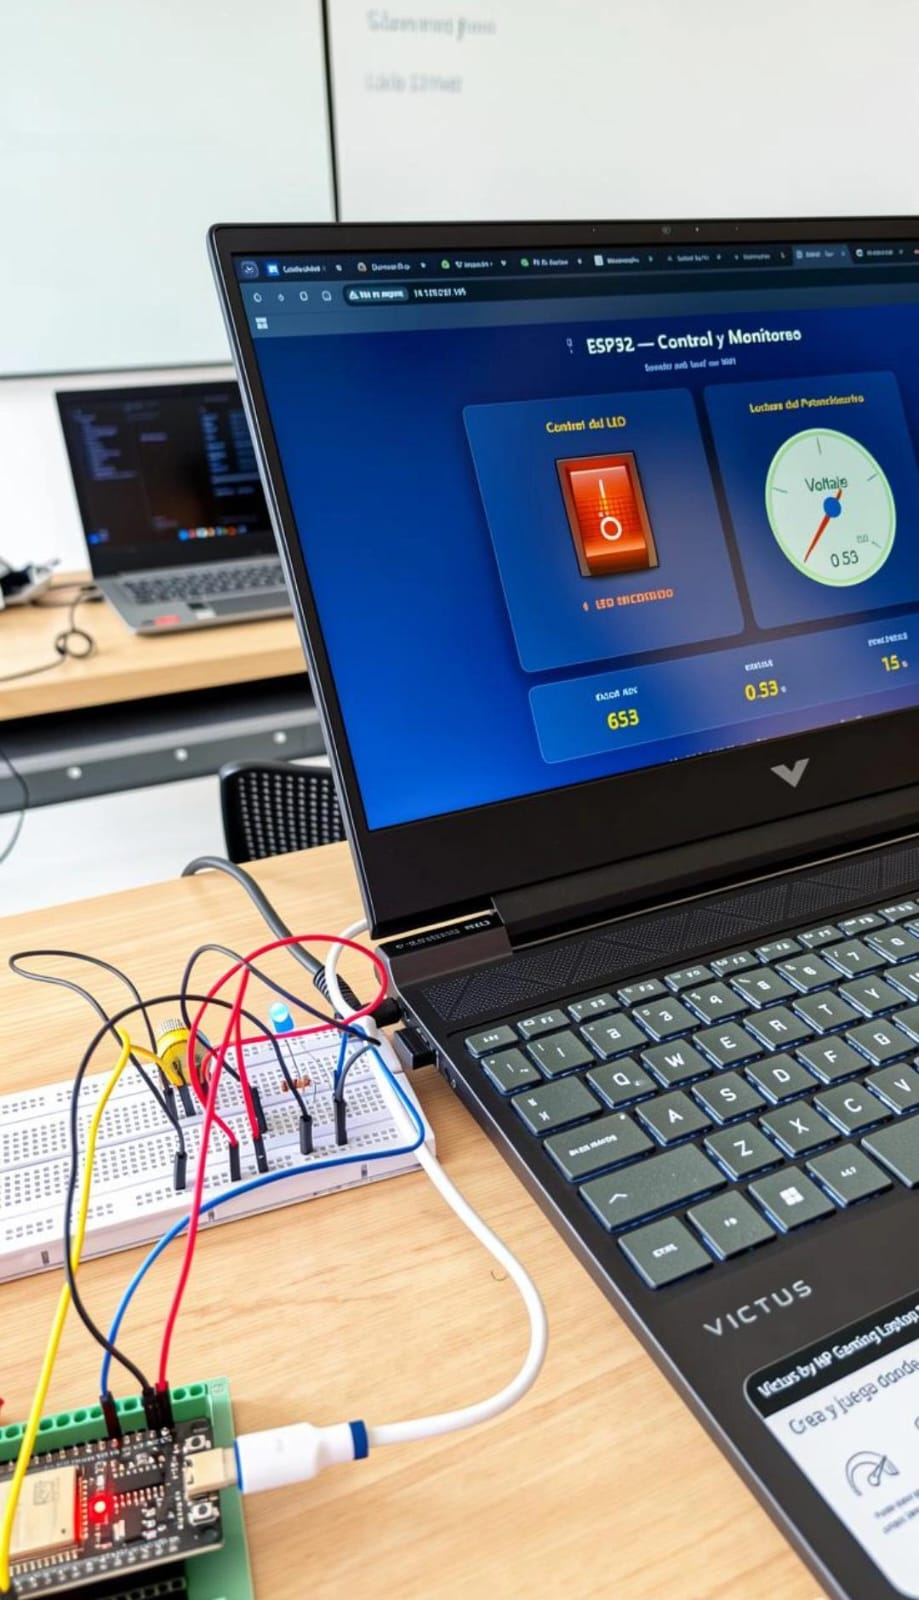
\includegraphics[width=\textwidth]{../Imagenes/Potenciometro_y_On_Off_Wifi_imgs/Potenciometro_y_On_Off_Wifi_img2.jpeg}
    \caption{Vista del montaje físico: laptop HP Victus mostrando la interfaz web con el LED encendido (estado rojo brillante), ESP32 conectado a la protoboard con el circuito del potenciómetro y LED.}
    \label{fig:wifi2}
\end{subfigure}
\caption{Interfaz web y montaje físico del proyecto WiFi}
\label{fig:montaje}
\end{figure}

En las Figuras~\ref{fig:wifi1} y~\ref{fig:wifi2} se puede observar:
\begin{itemize}
    \item La interfaz web presenta un diseño moderno con estética \textit{glassmorphism}: fondo con gradiente azul oscuro, paneles con bordes dorados semitransparentes y efecto de desenfoque.
    \item El interruptor del LED es un botón 3D estilo industrial con efectos de iluminación CSS que simulan un switch físico real.
    \item El gauge de Google Charts muestra el voltaje actual con zonas de color (verde/amarillo/rojo) y marcas de 0 a 3,3\,V.
    \item El panel inferior muestra tres valores numéricos en tiempo real: valor ADC crudo (0--4095), voltaje calculado en voltios, y porcentaje (0--100\%).
    \item En la imagen 1 se aprecia una gráfica de ``Voltaje del potenciómetro en el tiempo'' que registra el historial de lecturas.
    \item En la imagen 2 se ve el ESP32 conectado al computador vía USB, con los cables del circuito visibles en la protoboard.
\end{itemize}

% ══════════════════════════════════════════════════════════════
\section{Videos de Funcionamiento}
% ══════════════════════════════════════════════════════════════

Se dispone de un video que demuestra el funcionamiento completo del proyecto:

\begin{itemize}
    \item \textbf{Potenciometro\_y\_On\_Off\_Wifi\_Funcionamiento.mp4}: Demostración del sistema en funcionamiento, mostrando la interacción en tiempo real entre la página web y el circuito físico. Se observa cómo al girar el potenciómetro, el gauge y los valores numéricos se actualizan instantáneamente, y cómo al pulsar el interruptor virtual el LED se enciende y apaga en el circuito.
\end{itemize}

Este video se encuentra en la carpeta \texttt{Videos/Potenciometro\_y\_On\_Off\_Wifi\_vid/} del repositorio del proyecto.

% ══════════════════════════════════════════════════════════════
\section{Proceso de Creación}
% ══════════════════════════════════════════════════════════════

El desarrollo de este proyecto partió de los conceptos de los proyectos anteriores (potenciómetro básico y Bluetooth) y añadió la funcionalidad de servidor web WiFi:

\begin{enumerate}
    \item \textbf{Punto de partida:} Se tomaron los conceptos de lectura ADC y control de LED de los proyectos previos, pero se reemplazó la comunicación serial/Bluetooth por un servidor web HTTP.
    
    \item \textbf{Configuración WiFi:} Se añadieron las librerías \texttt{WiFi.h} y \texttt{WebServer.h}, configurando el ESP32 en modo estación para conectarse a la red local.
    
    \item \textbf{Diseño de la interfaz web:} Se creó una página HTML completa con CSS moderno (glassmorphism, gradientes, animaciones 3D) almacenada directamente en el código fuente usando \texttt{PROGMEM}.
    
    \item \textbf{Interruptor industrial CSS:} Se implementó un botón 3D con transformaciones CSS \texttt{perspective}, \texttt{rotateX} y animaciones de iluminación para simular un interruptor físico realista.
    
    \item \textbf{Integración de Google Charts:} Se incorporó la librería de Google Charts vía CDN para renderizar el gauge de voltaje con zonas de color y actualización en tiempo real.
    
    \item \textbf{API REST JSON:} Se diseñaron tres endpoints (\texttt{/}, \texttt{/datos}, \texttt{/led}) que permiten la comunicación asíncrona entre el navegador y el ESP32 usando la API Fetch de JavaScript.
    
    \item \textbf{Pruebas y validación:} Se verificó el funcionamiento accediendo a la IP del ESP32 desde el navegador, comprobando que el gauge se actualizara en tiempo real y que el LED respondiera correctamente al interruptor web.
\end{enumerate}

% ══════════════════════════════════════════════════════════════
\section{Diferencias con Proyectos Anteriores}
% ══════════════════════════════════════════════════════════════

\begin{table}[H]
\centering
\begin{tabular}{lccc}
\toprule
\textbf{Característica} & \textbf{Base} & \textbf{Bluetooth} & \textbf{WiFi (este)} \\
\midrule
Lectura ADC & \checkmark & \checkmark & \checkmark \\
Control del LED & PWM & PWM & On/Off digital \\
Monitoreo USB Serial & \checkmark & \checkmark & Solo para depuración \\
Comunicación inalámbrica & -- & Bluetooth SPP & WiFi HTTP \\
Interfaz de usuario & Monitor serial & App BT Terminal & Página web completa \\
Visualización gráfica & -- & -- & Gauge + gráfica tiempo \\
Acceso multidispositivo & -- & 1 celular & Cualquier navegador \\
Hardware adicional & -- & Ninguno & Ninguno \\
\bottomrule
\end{tabular}
\caption{Comparación entre los tres proyectos de potenciómetro}
\end{table}

% ══════════════════════════════════════════════════════════════
\section{Conceptos Técnicos Clave}
% ══════════════════════════════════════════════════════════════

\subsection{PROGMEM y Almacenamiento en Flash}

La directiva \texttt{PROGMEM} indica al compilador que almacene la cadena en la memoria Flash (programa) en lugar de la RAM. Esto es crucial porque la página web ocupa más de 16\,KB, y el ESP32 tiene solo 520\,KB de RAM pero 4\,MB de Flash.

\subsection{Raw String Literals en C++}

La sintaxis \texttt{R"=====( ... )=====" } permite incluir texto con comillas, saltos de línea y caracteres especiales sin necesidad de secuencias de escape. Esto es indispensable para embeber código HTML/CSS/JavaScript dentro del firmware de Arduino.

\subsection{Comunicación Asíncrona con Fetch API}

El navegador utiliza la API \texttt{fetch()} para realizar peticiones HTTP asíncronas al ESP32 sin recargar la página. Esto permite la actualización en tiempo real del gauge y los datos numéricos cada 500\,ms mediante \texttt{setInterval()}.

\subsection{Formato JSON para Intercambio de Datos}

El endpoint \texttt{/datos} devuelve un objeto JSON con tres campos:
\begin{verbatim}
    {"adc": 1123, "voltaje": 0.90, "porcentaje": 27}
\end{verbatim}

Este formato es parseado automáticamente por \texttt{fetch().then(r => r.json())} en el navegador.

% ══════════════════════════════════════════════════════════════
\section{Conclusiones}
% ══════════════════════════════════════════════════════════════

\begin{itemize}
    \item El proyecto demuestra cómo convertir el ESP32 en un servidor web IoT completo, sirviendo una aplicación web moderna con interfaz gráfica interactiva.
    \item La combinación de \texttt{WiFi.h} y \texttt{WebServer.h} permite implementar una API REST con apenas tres rutas, suficientes para control y monitoreo.
    \item El uso de \texttt{PROGMEM} y raw string literals permite almacenar páginas web completas (HTML+CSS+JS) en la Flash del ESP32 sin consumir RAM.
    \item La interfaz web con glassmorphism, interruptor 3D CSS y gauge de Google Charts ofrece una experiencia de usuario superior a las interfaces de texto serial o aplicaciones Bluetooth.
    \item La comunicación asíncrona con \texttt{fetch()} y JSON permite actualización en tiempo real cada 500\,ms sin recargar la página.
    \item A diferencia del Bluetooth (limitado a un dispositivo), el servidor WiFi permite acceso simultáneo desde múltiples dispositivos en la misma red.
    \item Este proyecto sienta las bases para aplicaciones IoT más avanzadas como domótica, monitoreo industrial remoto y sistemas SCADA a pequeña escala.
\end{itemize}

\end{document}
